
\begin{itemize}
  \item{
      MIE
    }
  \item{
      NN
    }
  \item{
      Input set 
    }
  \item{
    }
\end{itemize}

\section{Entropy and Mutual Information}

\paragraph{Entropy}-- quantifies information content of a random variable. It's
generally measured in bits and can be though of as the expected information
content when we sample a random variable once. Entropy for a discrete random
variable is defined in \autoref{eq:entropy}.

\begin{equation}
  H(X)=-\sum _{i=1}^{n}{P (x_{i})\log P(x_{i})}
\label{eq:entropy}
\end{equation}

Consider a random variable $X$ s.t $P(X=1) = P(X=0) = 0.5$, this tells
us that $H(X) = 1$ and every time we sample $X$ we are expected to gain 1 bit of
information.

Similarly for a random variable $Y$ s.t $P(X=0) = 0.5, P(X=1) = P(X=2) = 0.25$,
we have $H(Y) = 1.5$

\paragraph{Conditional Entropy}-- quantifies the amount of information needed to
describe an outcome of variable $Y$ given that value of another random variable
$X$ is already known. Entropy of $Y$ given $X$ is written as $H(Y|X)$.
Conditional Entropy for a discrete random variable is defined in
\autoref{eq:condEntropy}

\begin{equation}
H(Y|X)\ =-\sum _{x\in {X},y\in {Y}}p(x,y)\log {\frac {p(x,y)}{p(x)}}
\label{eq:condEntropy}
\end{equation}

Consider a random variable pair $X$ and $Y$ s.t 
$$P(X=0,Y=0) = P(X=0,Y=1) = 0.25, P(X=1,Y=0) = 0.5, P(X=1,Y=1) = 0$$
then $H(Y|X) = 0.5$ and $H(X|Y) \approx 0.6887$, while $H(X) = 1$ and $H(Y)
\approx 0.8112$

\paragraph{Mutual Information (MI)}-- is a measure between two random variables,
it builds on top of entropy and measures how much information the variables have
in common. It quantifies information gained about one variables when observing
the other. Mutual information is generally computed either explicitly using the
probabilities as in \autoref{eq:miExplicit} or using entropies as in
\autoref{eq:miEntropy}.

\begin{equation}
      I(X,Y)=\sum _{y\in Y}\sum _{x\in X}{p(x,y)\log {\left({\frac
      {p(x,y)}{p(x)\,p(y)}}\right)}} 
\label{eq:miExplicit}
\end{equation}

\begin{equation}
  I(X, Y) = H(X) - H(X|Y)
\label{eq:miEntropy}
\end{equation}

Consider the random variables $X$ and $Y$ as before in the conditional entropy
section. 
$$P(X=0,Y=0) = P(X=0,Y=1) = 0.25, P(X=1,Y=0) = 0.5$$
Here we can see that $I(X,Y) \approx 0.3113$

\section{Neural Network}

\paragraph{Neural Network} is a machine learning framework based on multiple
perceptrons which are usually connected in sequential layers as in
\autoref{fig:neuralNetworkEX}. However for our purposes we can define the neural
network to be an abstract collection of parameterized functions.

\begin{figure}[H]
  \centering
  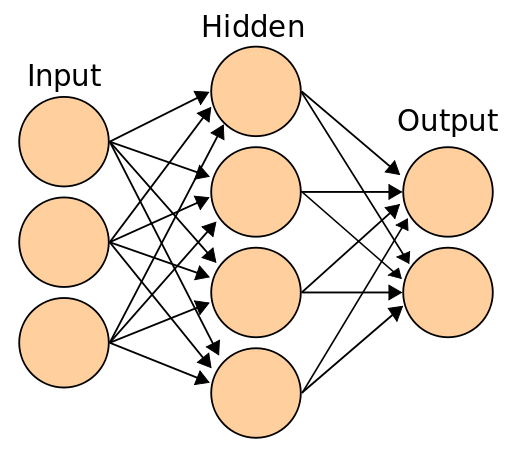
\includegraphics[width=0.35\textwidth]{figs/neural_network_ex.png}
  \caption{
    https://commons.wikimedia.org/wiki/File:Artificial\_neural\_network.svg
  }
  \label{fig:neuralNetworkEX}
\end{figure}

\paragraph{Neural Network} is a machine learning framework, based on
individually connected perceptrons

A neural network is a machine learning framework

---------------------------------------------------------------


Before developing a plan for how we are going to realize the project in code we
needed to fully understand the ideas presented in the paper:
\begin{itemize}
    \begin{item}
      We needed to identify the main ideas of the paper and understand why some
      parts of the paper are not agreed upon in the scientific community.
      Understand why his ideas are contentious and whether reproducing his
      experiments could bring more validity to his claims. This involved reading
      papers published by Tishby and academics who shown an opposing view to
      him.
    \end{item}
    \begin{item}
      A main tool that the paper relies on is MIE (Mutual Information
      Estimation). Reading about MIE we quickly understood that MIE is a
      contentious part of the project as a result we had to do a decent amount
      of research regarding the subject. MIE is difficult because we are trying
      to estimate information between two continuous distributions using only a
      discrete sample set. This area has not seen much academic attention so the
      tools we ended up using could be greatly improved in the future.
    \end{item}
\end{itemize}

Once we had a reasonable understanding of the ideas in the paper and which areas
needed more attention we diverted our attention to figuring out the details of
how the experiments were conducted figure out what hyper parameters Tishby
decided are important and what assumptions he made whilst devising the
experiments. 

In addition we needed to find out what resources are available to us online,
what programming frameworks we are going to use for the projects implementation,
and to think about possible extensions to the project once the success criteria
has been achieved.

\begin{itemize}
  \item{
      Online Resources: The two main papers by Tishby and by Saxe have made
      their code public online via Github, we made 

      Online Resources: The two main papers we were looking at has made their
      code available to the public via Github, the papers are Tishby's paper and
      the main opposing paper by Saxe.
    }
  \item{
      Programming frameworks: The original experiment implementation by Tishby
      has used the Tensorflow framework. We have decided to use the Keras
      framework as it produces code that is more concise and is easier to
      read/maintain. Furthermore rewriting the experiments in a different
      framework means that we cannot rely on the details of Tishby's and
      potentially avoid any mistakes that may exist in the original
      implementation.
    }
    \begin{item}

      Thinking about how we could extend the project helped us understand the
      scope of the project and what areas were most important and/or interesting
      to us. 

      We came up with a couple of extensions before having written any code but
      the most interesting one only materialized after a good deal amount of
      work into the project (that is the AS-IF-Random experiment described
      below)

      \begin{itemize}
        \item{
            Different Datasets : the most straight forward extension to the
            project just using different dataset to the one Tishby used. This is
            essentially just varying one of the parameters in the Neural
            Network. (Implemented)
          }
        \item{
            Quantized Neural Network : the idea behind this was to only allow
            single neurons to acquire values in a given range say 1...256. This
            would make the distribution within a DNN later discrete and hence it
            would make calculating mutual information straightforward. (Not
            Implemented)
          }
        \item{
            As-If-Random : one problem with Tishby's work is that he calculates
            mutual information for a single epoch at a time which by definition
            is zero (in his paper he tries to justify the result will explore
            this later) this extension tries to explore the weights of a neural
            network as random variables by calculating mutual information for
            multiple epochs at a time.
          }
      \end{itemize}
    \end{item}
\end{itemize}



